\chapter{Commande proportionnelle intégrale d'un drone convertible à 6 degrés de liberté}
\minitoc

\section{Schéma de commande linéaire proportionnel intégral : 6 Dof}
\section{Integral-based linear control}
\label{sec:6dofcmd}
\subsection{Description of the control scheme}
\label{sec:ctl_sche}

A careful inspection of the control and the disturbance input matrices $\boldsymbol{G}_{w}$ and $\boldsymbol{E}_{w}$ in model \eqref{eq:lpv_linearisation} (see the output of Algorithm~\ref{alg:linea}) suggests an effective control architecture to reject a constant wind disturbance $\boldsymbol{w}$. Indeed, the ailerons and the propellers can be used symmetrically to generate respectively a moment about the $y_{[\text{b}]}$ axis, verifying equation \eqref{eq:momenty} and a force along the $x_{[\text{b}]}$ axis, verifying equation \eqref{eq:forcex}, thus compensating for the disturbance effect. Nevertheless, there is still a force along the $z_{[\text{b}]}$ axis to be compensated for by verifying equation \eqref{eq:forcez}, and an integral action can asymptotically converge to the desired force, even with a non-measured wind disturbance $\boldsymbol{w}$. We may thus stabilize the UAV at a hovering equilibrium as characterized in Theorem~\ref{thm:eqs}. Since we don't measure the wind $\boldsymbol{w}$, the values of $\psi$ and $\theta$ in Algorithm~\ref{alg:eq} are unknown. The proposed controller, shown in Fig.~\ref{fig:commande_int}, uses integral action to obtain these two unknown angles. Its feedback loop involves the following error variables output, which should converge to zero in any hovering position:
\begin{align}
  \boldsymbol{e}_{p}= \boldsymbol{r}_{p} - \boldsymbol{p}, \; \boldsymbol{e}_{v \epsilon \omega} = -  
     \left[ \begin{smallmatrix} \mathbb{I}_{3}  & \mathbb{0}_{3\times 1} & \mathbb{0}_{3\times 2} & \mathbb{0}_{3}\\
     \mathbb{0}_{1\times 3}  & 1 & \mathbb{0}_{1\times 2} & \mathbb{0}_{1 \times 3} \\
         \mathbb{0}_{3}  & \mathbb{0}_{3\times 1} & \mathbb{0}_{3\times 2} &   \mathbb{I}_{3}
         \end{smallmatrix} \right]
  \smallmat{
         \tilde{\boldsymbol{v}} \\
         \tilde{\boldsymbol{\epsilon}} \\
         \tilde{\boldsymbol{\omega}}_{\text{b}} 
     },
\label{eq:error_var}
\end{align}    
where $\boldsymbol{r}_{p} \in \mathbb{R}^{3}$ is the constant position reference comprising a target position for the translational motion (note that $\boldsymbol{r}_{p}$ is the reference input to the control scheme).

The error variables in \eqref{eq:error_var} can be represented as in the block diagram of Fig.~\ref{fig:commande_int} by defining 
the output $\boldsymbol{y}\in \real^{10}$ of the linearized plant dynamics \eqref{eq:lpv_linearisation}, having the incremental state vector $\boldsymbol{\tilde{x}} \in \real^{10 \times 1}$, as follows
\begin{align}
    \label{eq:output_lin}
    \boldsymbol{y} = \boldsymbol{C} \boldsymbol{\tilde{x}} + \smallmat{\boldsymbol{p}_{\mathrm{eq}} \\ \mathbb{0}_{7 \times 1}}, \quad
 \boldsymbol{C} := \smallmat{\mathbb{I}_{6} & \mathbb{0}_{6\times 1} & \mathbb{0}_{6\times 2} &\mathbb{0}_{6\times 3}\\
    \mathbb{0}_{1\times 6} & 1 & \mathbb{0}_{1\times 2} &\mathbb{0}_{1\times 3}\\
    \mathbb{0}_{3\times 6} & \mathbb{0}_{3\times 1} & \mathbb{0}_{3\times 2} &  \mathbb{I}_{3}
},
\end{align}
where  the output matrix $\boldsymbol{C} \in \real^{10\times12}$ removes the $\tilde{\epsilon}_{2}$ and $\tilde{\epsilon}_{3}$ components from the state vector $\tilde{\boldsymbol{x}}$. 
% \begin{align*}
%      \boldsymbol{S} = \left[ \begin{smallmatrix} \mathbb{I}_{3} & \mathbb{0}_{3\times 1} & \mathbb{0}_{3\times 1} & \mathbb{0}_{3\times 2} & \mathbb{0}_{3}\\
%      \mathbb{0}_{1\times 3} & 0 & 1 & \mathbb{0}_{1\times 2} & \mathbb{0}_{1 \times 3} \\
%          \mathbb{0}_{3} & \mathbb{0}_{3\times 1} & \mathbb{0}_{3\times 1} & \mathbb{0}_{3\times 2} &   \mathbb{I}_{3}
%          \end{smallmatrix} \right], 
% \end{align*}



% \begin{align*}
%      \boldsymbol{e}_{p}= \boldsymbol{r}_{p} - \boldsymbol{p}, \quad \boldsymbol{e}_{v \epsilon \omega} = -\boldsymbol{S} \smallmat{
%          \boldsymbol{v} \\
%          \boldsymbol{q} \\
%          \boldsymbol{\omega}_{\text{b}} 
%      }, \\
%      \boldsymbol{S} = \left[ \begin{smallmatrix} \mathbb{I}_{3} & \mathbb{0}_{3\times 1} & \mathbb{0}_{3\times 1} & \mathbb{0}_{3\times 2} & \mathbb{0}_{3}\\
%      \mathbb{0}_{1\times 3} & 0 & 1 & \mathbb{0}_{1\times 2} & \mathbb{0}_{1 \times 3} \\
%          \mathbb{0}_{3} & \mathbb{0}_{3\times 1} & \mathbb{0}_{3\times 1} & \mathbb{0}_{3\times 2} &   \mathbb{I}_{3}
%          \end{smallmatrix} \right], 
% \end{align*}
 % $\boldsymbol{S} \in \real^{7 \times 10}$ is an output selection matrix, which removes $\eta$, $\epsilon_{2}$ and $\epsilon_{3}$ component from the measured output. 
% We introduce $\boldsymbol{r} \in \real^{10 \times 1}$ as an input disturbance vector defined by $\boldsymbol{r} = \smallmat{\boldsymbol{r}_{p} \\ \boldsymbol{r}_{v \epsilon \omega}}$.
\begin{figure}[t!]
    \centering
    %\includegraphics[trim=7cm 0cm 2.5cm 1cm,clip,width=1\columnwidth]{figure/commande_integrale.png}
    \includegraphics[width=1\columnwidth]{figures/commande_integrale.png}
    \caption{Proposed integral-based controller with the wind perturbation $\boldsymbol{w}$, a plant-input perturbation $\boldsymbol{d}$ and a plant-output perturbation $\nu$.}
    \label{fig:commande_int}
\end{figure}
As shown in Fig.~\ref{fig:commande_int}, the controller dynamic equations are based on the measured error $\boldsymbol{e}$ as follows
\begin{multline}
\label{eq:contoller}
    \boldsymbol{e} = \smallmat{
        \boldsymbol{e}_{p}^\top & \boldsymbol{e}_{v\epsilon\omega}^\top}^\top, \quad \dot{\boldsymbol{x}}_{c} = \boldsymbol{H} \boldsymbol{e}, \quad    \boldsymbol{u} = \boldsymbol{\Sigma} \boldsymbol{x}_{c} + \boldsymbol{u}_{K},\\
    \boldsymbol{\Sigma} := \begin{bmatrix} \! 1 \!&\! 1\! & \!0\! &\! 0\!\\ \!0\! & \!0\! & \!1 \!& \!1\!\end{bmatrix}^\top, \quad
    \boldsymbol{u}_{K} = \frac{n_1 s+n_0}{d_2 s^{2}+d_1 s + d_0}\boldsymbol{K} \boldsymbol{e} ,
\end{multline}
where $\boldsymbol{x}_{c} \in \mathbb{R}^{2}$ is the integral action state; $\boldsymbol{\Sigma}$ is an input allocation matrix that allows assigning the first component of the integrator state to the propellers action and the second component to the elevons action. Scalars $n_1$, $n_0$,  $d_2$,  $d_1$,  $d_0$ are respectively the numerator and denominator coefficients of a filter used to avoid a direct input-output transmission that would amplify high-frequency measurement noise. This filter induces a strictly proper controller, for increased robustness to additive uncertainties. We define the controller $\boldsymbol{F}$ having dimensions 4\texttimes10 having transfer matrix $\boldsymbol{F}(s) = T_{\boldsymbol{e} \rightarrow \boldsymbol{u}}(s)$ as described in \eqref{eq:contoller} and interconected as in Fig.~\ref{fig:commande_int}. The plant $\boldsymbol{P}$ having dimensions 10\texttimes4 represents the linearized DarkO dynamics. The output of the plant $\boldsymbol{y} \in \real^{10\times1}$ is used as the input of controller $\boldsymbol{F}$.

% According to the discussions in Section~\ref{subsec:LinWind}, the quaternion linearization evolves in ${\mathbb R}^3$, therefore when $\boldsymbol{P}$ represents the linearized plant dynamics \eqref{eq:lpv_linearisation}, having the incremental state vector $\boldsymbol{\tilde{x}} \in \real^{10 \times 1}$, the output $\boldsymbol{y}$ can be obtained by 
% \begin{align}
%     \label{eq:output_lin}
%     \boldsymbol{y} = \smallmat{\mathbb{I}_{6} & \mathbb{0}_{6\times 1} & \mathbb{0}_{6\times 2} &\mathbb{0}_{6\times 3}\\
%     \mathbb{0}_{1\times 6} & 1 & \mathbb{0}_{1\times 2} &\mathbb{0}_{1\times 3}\\
%     \mathbb{0}_{3\times 6} & \mathbb{0}_{3\times 1} & \mathbb{0}_{3\times 2} &  \mathbb{I}_{3}
% } = \boldsymbol{C} \boldsymbol{\tilde{x}}.
% \end{align}
% where $\boldsymbol{C} \in \real^{10\times12}$ is the output matrix.

In view of the symmetries of the actuators on the UAV, we have constrained the structure of matrix $\boldsymbol{K}$ in \eqref{eq:contoller}, associated with the controller's proportional action, in order to use the actuators in a physically meaningful way as follows:
\begin{align}
\label{eq:k_struct}
    \!\!\!\boldsymbol{K}_{\text{struct}} \!=\!  \smallmat{
             k_{1}& \shortminus k_{2}& k_{3}&  k_{4}& \shortminus k_{5}&  k_{6}& \shortminus k_{7}&  k_{8}&  k_{9}& \shortminus k_{10}\\
             k_{1}&  k_{2}& k_{3}&  k_{4}&  k_{5}&  k_{6}&   k_{7}& \shortminus k_{8}& \shortminus k_{9}&  k_{10}\\
            \shortminus k_{11}& \shortminus k_{12}& k_{13}& \shortminus k_{14}& \shortminus k_{15}& \shortminus k_{16}&   k_{17}& \shortminus k_{18}&  k_{19}& \shortminus k_{20}\\
            \shortminus k_{11}&  k_{12}& k_{13}& \shortminus k_{14}&  k_{15}&  k_{16}&   \shortminus k_{17}&  k_{18}&  k_{19}&  k_{20} 
         }.
\end{align}
In particular, a position error on the $z_{[\text{i}]}$ axis of the NED world frame (see Fig.~\ref{fig:darko2}) results in a symmetric use of the two propellers that generates a force along the $x_{[\text{b}]}$ axis of the UAV. The symmetric use of the two motors is reflected by the same-sign in coefficients $k_{3}$ and $k_{6}$ on columns 3 and 6 of $\boldsymbol{K}$, corresponding respectively to the position and velocity errors on the $z_{[\text{i}]}$ axis. Similarly, a position or speed error along the drone's lateral axis $y_{[\text{b}]}$ will be compensated for by an antisymmetric use of the motors, as reflected by the coefficients $k_{2}$ and $k_{5}$ and their opposite signs on columns 2 and 5 of $\boldsymbol{K}$. An angular velocity error about the  $x_{[\text{b}]}$ axis must be compensated for by an antisymmetric use of the elevons, as reflected by coefficient $k_{18}$ having opposite signs on column 8 of $\boldsymbol{K}$. Parallel arguments explain the remaining coefficients of matrix $\boldsymbol{K}$ in \eqref{eq:k_struct}. An advantage of the structure in \eqref{eq:k_struct} is the reduction of the number of variables to be optimized, from 40 to 20 scalar gains.


The closed loop shown in Fig.~\ref{fig:commande_int}, is an output feedback with 10 outputs, consisting of the three linear positions, the three linear velocities, one of the three attitude angles ($\epsilon_{1}$) and the three angular velocities. This structure can be seen as a MIMO proportional-integral feedback. The parameters to be tuned in controller $\boldsymbol{F}$ \eqref{eq:contoller} are the proportional gain $\boldsymbol{K} \in \real^{4\times10}$ in \eqref{eq:k_struct}, the integral gain $\boldsymbol{H} \in \real^{2\times10}$ and the filter parameters $n_1$, $n_0$,  $d_2$,  $d_1$,  $d_0$, as highlighted in yellow in Fig.~\ref{fig:commande_int}. A suitable tuning method should ensure desirable disturbance rejection and satisfactory robustness to unmodeled dynamics. These two goals lead to a trade-off because disturbance rejection requires an aggressive tuning while robustness properties are ensured by a frequency roll-off strategy. We discuss next two optimization-based tuning methods. The first one is issued from the ideas proposed in \cite{SANSOUACA}, which did not need the linearized dynamics of Theorems~\ref{thm:eqs} and~\ref{th:lin}, and is summarized in Section~\ref{sec:zerowind}. It is a multi-objective synthesis with $H_{\infty}$ constraints based on the zero-wind model discussed in Remarks~\ref{rk:zerowindmodel} and~\ref{rk:zerolin} and derived in \cite{SANSOUACA}. We will show that this first method fails to stabilize the drone in certain wind ranges, due to the lack of knowledge of the dynamics characterized in Theorems~\ref{thm:eqs} ans~\ref{th:lin}. The second tuning method, presented in Sec.\ref{sec:h_inf_multi}, is an iterative multi-objective synthesis with $H_{\infty}$ constraints, based on a collection of models associated with different wind conditions and derived based on Theorems~\ref{thm:eqs} and~\ref{th:lin}, through Algorithms~\ref{alg:eq} and~\ref{alg:linea}.
\begin{table}[ht]
\centering
\begin{tabular}{|c|c|c|} 
\hline
Measurement & Value & Units\\
 \hline
 $\boldsymbol{p}$ & \SI{2.5e-4}{} & \SI{}{\meter}  \\ 
 \hline
  $\tilde{\boldsymbol{v}}$  & \SI{1.2e-3}{} &  \SI{}{\meter\per\second}  \\ 
  \hline
  $\tilde{\boldsymbol{\epsilon}}$ & \SI{4.7e-4}{} &  \\
  \hline
  $\tilde{\boldsymbol{\omega}}_{\text{b}}$ & \SI{2.7e-3}{} &\SI{}{\radian\per\second}\\
 \hline
\end{tabular}
\caption{\label{tab:sim_noise} Standard deviation of the modeled sensor noise added to the simulated measurements.}
\label{tab:noise}
\end{table}
In our numerical validation, reported in Sections~\ref{sec:zerowind} and~\ref{sec:h_inf_multi} (see in particular Fig.~\ref{fig:SimSytuneStruct_zero} and Fig.~\ref{fig:SimSytuneStruct_lpv}),
measurement noise is added to the output to produce practically reasonable numerical results.
%all the sensors used to obtain the UAV's output vector $\boldsymbol{y}$. 
The standard deviations of the adopted noise levels are reported in Table~\ref{tab:noise}.
Moreover,
in addition to reporting the simulation results of the linear feedback of Fig.~\ref{fig:commande_int} with the linearized model \eqref{eq:lpv_linearisation}, 
in Sections~\ref{sec:zerowind} and~\ref{sec:h_inf_multi},
we also simulate the closed loop by replacing the linearized plant $\boldsymbol{P}$ with the 
% Simulations (Fig.~\ref{fig:SimSytuneStruct_zero} and Fig.~\ref{fig:SimSytuneStruct_lpv}) were performed with the 
nonlinear model \eqref{eq:dyna_orig} including many real-world effects.
When replacing the linearized plant with the nonlinear dynamics \eqref{eq:dyna_orig}, whose state is $\boldsymbol{x} = (\boldsymbol{p}, \boldsymbol{v},
         \boldsymbol{q},
         \boldsymbol{\omega}_{\text{b}}) \in \real^{13} $,
we replace the linear output $\boldsymbol{y}$ with the following surrogate nonlinear version
% We derive the output vector $\boldsymbol{y}_{\text{NL}} \in \real^{10 \times 1}$ from the non-linear state vector $\boldsymbol{x}$  to feedback the nonlinear model \eqref{eq:dyna_orig} with the controller \eqref{eq:contoller}.
\begin{align}
\label{eq:output}
    \boldsymbol{y}_{\text{NL}} \!=\! \smallmat{\boldsymbol{p}\\
     \boldsymbol{v}\\
     \epsilon_{1}\\
     \boldsymbol{\omega}_{\text{b}}} \!=\! \left[ \begin{smallmatrix} \mathbb{I}_{6} & \mathbb{0}_{6\times 1} & \mathbb{0}_{6\times 1} & \mathbb{0}_{6\times 2} & \mathbb{0}_{3}\\
     \mathbb{0}_{1\times 3} & 0 & 1 & \mathbb{0}_{1\times 2} & \mathbb{0}_{1 \times 3} \\
         \mathbb{0}_{3} & \mathbb{0}_{3\times 1} & \mathbb{0}_{3\times 1} & \mathbb{0}_{3\times 2} &   \mathbb{I}_{3}
         \end{smallmatrix} \right]
         \smallmat{\boldsymbol{R}^\top_{\psi}\boldsymbol{p} \\ \boldsymbol{R}^\top_{\psi}\boldsymbol{v} \\
\boldsymbol{q}_{\mathrm{eq}\psi}^{-1} \otimes \boldsymbol{q} \\
         \boldsymbol{\omega}_{\text{b}}  }.
\end{align}
% However, it is not possible to form the output vector $\boldsymbol{y}$ without knowledge of the wind direction in the horizontal plane linked to the rotation $\boldsymbol{R}^\top_{\psi}$ ensuring that the drone is facing into the wind. As we don't have access to the wind measurement, we chose to use the drone's current orientation along the $z_{[\text{i}]}$ axis to rotate the $\boldsymbol{p}$ position and $\boldsymbol{v}$ velocity measurements. To do this, we have $\boldsymbol{R}^\top_{\psi} = \boldsymbol{R}(\smallmat{\cos(\frac{\psi}{2}) & 0 & 0 & \sin(\frac{\psi}{2})})$ where { \color{red}$\psi$ doit on garder cette nottation} is the UAV's orientation along the $z_{[\text{i}]}$ axis. We don't need to worry about quaternion rotation $\boldsymbol{q}_{\mathrm{eq}\psi}^{-1}$, as the selection matrix (see \eqref{eq:output}) removes the quaternion components linked to rotation around $z_{[\text{i}]}$ axis. 
% { \color{red}This solution is linked to the fact that the controller has a certain stability domain, so the drone must be close enough to the equilibrium point for the control law to converge.}


In the next sections we denote the modulus margin of a transfer matrix $s \mapsto T_{v \rightarrow z}$ as $\Delta_m(T_{v \rightarrow z}) = \min\limits_{\omega\in R} \sigma_{\min}(T_{v \rightarrow z}(j\omega))$.

\begin{figure}[b!]
    \centering
    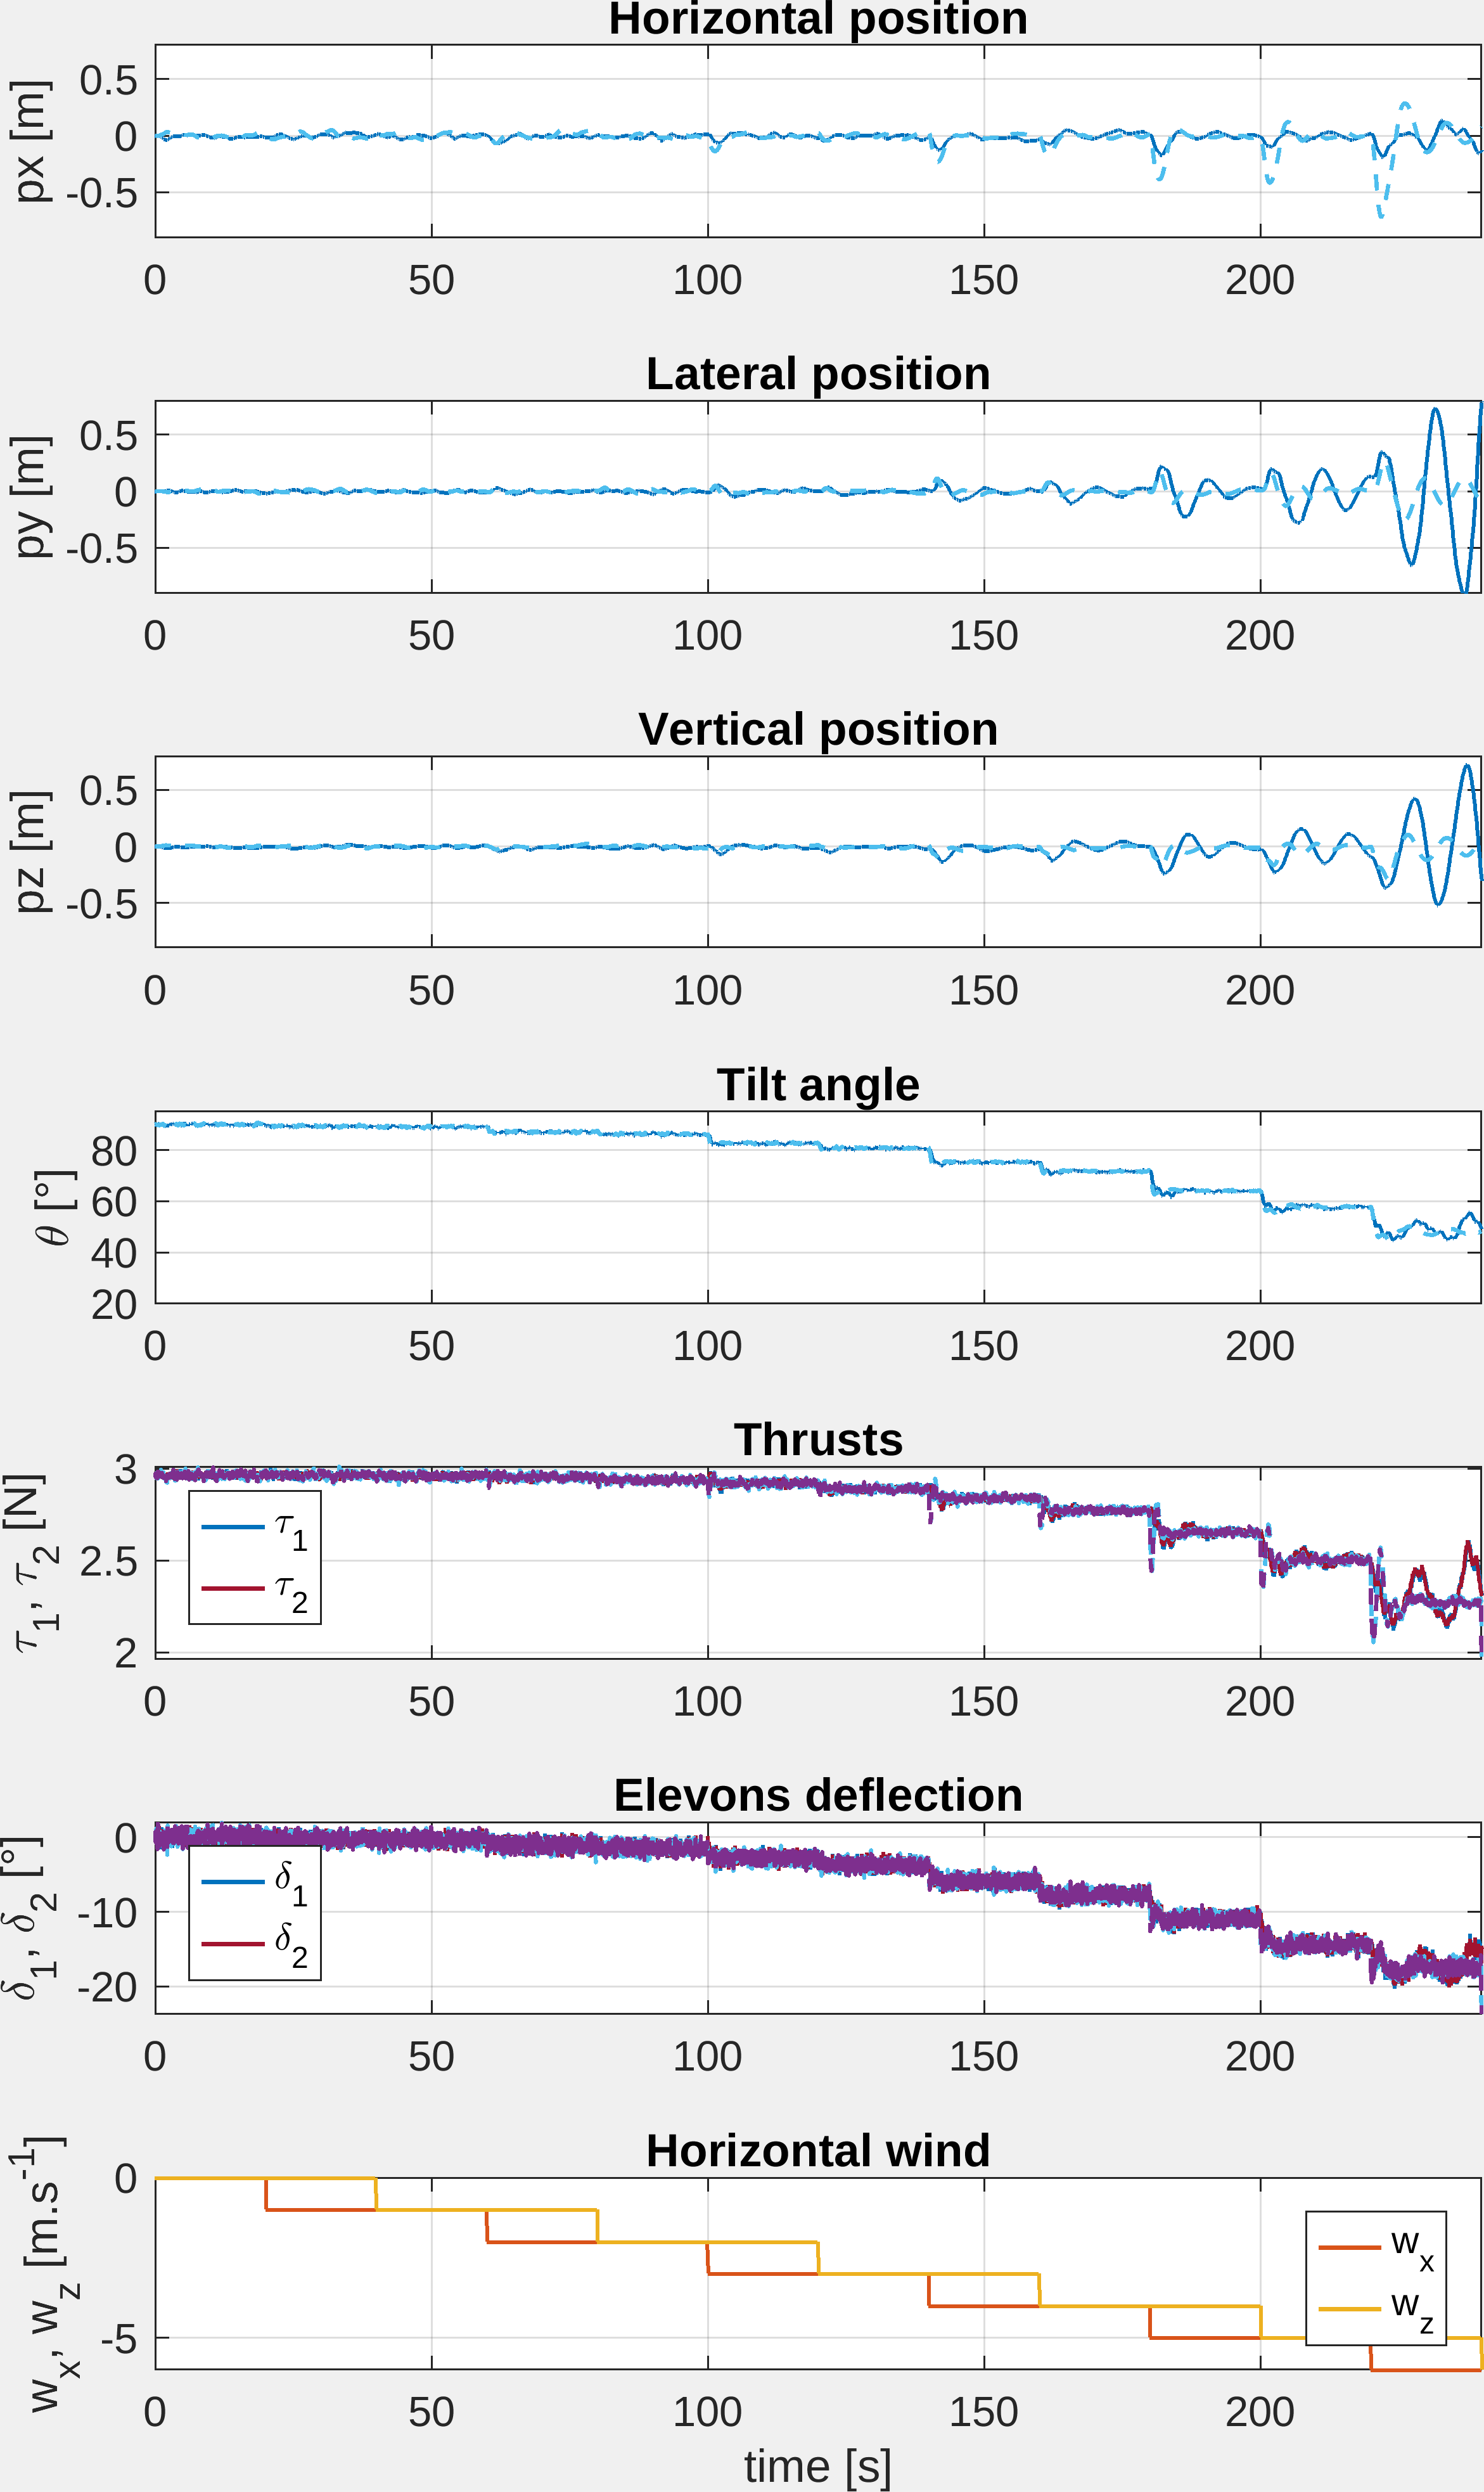
\includegraphics[trim=0cm 0cm 0cm 0cm,clip,width=0.9\columnwidth]{figures/sim_systune_zero_wind.png}
    \caption{Simulation of the non-linear model \eqref{eq:dyna_orig} (solid line) and the linearized model \eqref{eq:lpv_linearisation} (dashed line) with increasing constant wind steps with the controller tuned using the zero-wind optimization of Section~\ref{sec:zerowind}.}
    \label{fig:SimSytuneStruct_zero}
\end{figure}

\subsection{\texorpdfstring{Zero-wind $H_{\infty}$}{H {infty}}-based controller tuning }
\label{sec:zerowind}
For tuning the controller based on the zero wind, we use the linear plant model detailed in Remark~\ref{rk:zerolin}, $\boldsymbol{P}(s) = T_{\boldsymbol{u} \rightarrow \boldsymbol{y}}(s)$, obtained from equations \eqref{eq:linearized} and \eqref{eq:output_lin} as
\begin{align*}
    \boldsymbol{P}(s) = \boldsymbol{C} (s \mathbb{I}_{12} - \boldsymbol{A}_{0})^{-1} \boldsymbol{G}_{0}.
\end{align*} 
With reference to Fig.~\ref{fig:commande_int}, we introduce transfer matrices that correspond to robustness objectives: the output sensitivity function as $T_{\nu \rightarrow e}=(\mathbb{I}_{10}+\boldsymbol{P}\boldsymbol{F})^{-1}$ having dimensions 10\texttimes10, so that, $\lVert T_{\nu \rightarrow e} \rVert_{\infty}=\Delta_m(T_{\nu \rightarrow e})^{-1} $
and the input sensitivity function $T_{d \rightarrow u}=(\mathbb{I}_{4}+\boldsymbol{F}\boldsymbol{P})^{-1}$ having dimensions 4\texttimes4, so that $\lVert T_{d \rightarrow u} \rVert_{\infty}=\Delta_m(T_{d \rightarrow u})^{-1}$.
Consequently, the minimization of the  $H_{\infty}$-norm of $T_{\nu \rightarrow e}$ or $T_{d \rightarrow u}$, corresponds to increasing the input and output modulus margins. Since plant $\boldsymbol{P}$ is MIMO, we give importance to both the input and the output sensitivity functions which do not coincide, because $\boldsymbol{P}$ and $\boldsymbol{F}$ do not commute.
%
We also define the transfer matrix $T_{\nu \rightarrow u}$ having dimensions 4\texttimes10 linked to the impact of the measurement noise $\nu$ on the control input $\boldsymbol{u}$, and $T_{d \rightarrow y}$ having dimensions 10\texttimes4 representing the impact of the input disturbance $\boldsymbol{d}$ on the plant output $\boldsymbol{y}$. 
We solve the same problem as in our preliminary work \cite[eqn. (13)]{SANSOUACA} using the {\tt Systune} software \cite{1576856}, however we use the control diagram presented in section~\ref{sec:ctl_sche} which includes a filter on the proportional action and a different number of outputs. We also include in the plant $\boldsymbol{P}$ the linear actuators dynamics discussed in Remark~\ref{rem:saturation}.

Successive steps of increasing horizontal and vertical wind intensity (ranging from zero to \SI{-6}{\meter\per\second}) are applied, as shown in the lower plot of Fig.~\ref{fig:SimSytuneStruct_zero}. The selected wind pairs $(w_{x}, w_{z})$ are represented by red dots on the surfaces in Fig.~\ref{fig:saturation}, where we can see that the equilibrium $(\boldsymbol{u}_{\text{eq}}, \boldsymbol{x}_{\text{eq}})$ is reached without saturating the actuators. We only focus on the negative part of the vertical wind speed because it is the most limiting one. Indeed, the drone is lifted by the rising vertical wind (whose sign is negative in the NED frame), so it needs less traction on the propellers to compensate for the gravity. The motors generate less airflow over the elevons, which reduces their efficiency, leads to saturation, and destabilizes the drone.
The aim of the control system is to keep the UAV at the hovering position (defined as $\boldsymbol{r}_{p} = [0,0,0]^\top$), despite the increasing horizontal and vertical wind $w_{x}$ and $w_{z}$. Fig.~\ref{fig:SimSytuneStruct_zero} both linear simulations with the linearized plant dynamics \eqref{eq:lpv_linearisation} (dashed) and nonlinear simulations with the accurate model \eqref{eq:dyna_orig} (solid). Both the linear and nonlinear simulations consistently show that the controller performs well at low wind speed (in fact, the tuning is performed based on the zero-wind model). However, when the wind speed $w_{x}$ and $w_{z}$ exceed \SI{-5}{\meter\per\second}, the hovering position becomes unstable and the drone oscillates and diverges. The tilt angles $\theta$ are used to represent the attitude to give a better insight of the vehicle behavior, however the nonlinear simulation of the nonlinear dynamics \eqref{eq:dyna_orig} is carried out with unit quaternions. The instability observed in the simulation results of Fig.~\ref{fig:SimSytuneStruct_zero} confirms the experimental instabilities reported in \cite{SANSOUACA} where we used this same tuning method, and confirms the importance of Theorems~\ref{thm:eqs} and~\ref{th:lin} in Section~\ref{sec:model}, for an appropriate tuning of the controller gains, which is performed in the next section.

\subsection{\texorpdfstring{Multimodel $H_{\infty}$}{H {infty}}-based controller tuning}
\label{sec:h_inf_multi}

The simulation results obtained with the zero-wind tuning method (see Fig.~\ref{fig:SimSytuneStruct_zero}) together with the experimental instabilities observed in \cite{SANSOUACA} confirm the need for a controller gain tuning procedure exploiting the parametrized non-zero wind linearizations of Theorems~\ref{thm:eqs} and~\ref{th:lin}. Focusing again on the control scheme of Fig.~\ref{fig:commande_int}, we now explicitly consider the (linearized) wind effect on the plant, and we consider the linearized plant dynamics \eqref{eq:lpv_linearisation} with output \eqref{eq:output_lin} and with the selections in Algorithm~\ref{alg:linea} as
\begin{align*}
\label{eq:Pw_synthesis}
\numberthis
    \boldsymbol{P}_w(s) &= \begin{bmatrix}
        \boldsymbol{P}_{u}(s;w) &  \boldsymbol{P}_{w}(s;w)
    \end{bmatrix}\\&:= \boldsymbol{C} (s \mathbb{I}_{12} - \boldsymbol{A}_{w})^{-1} \begin{bmatrix}\boldsymbol{G}_{w} &   \boldsymbol{E}_{w}\end{bmatrix},
\end{align*}
whose input is the concatenation of the control input $\boldsymbol{u}$ and the wind disturbance input $\boldsymbol{w}$. As the model depends on the wind speed $\boldsymbol{w}$, we introduce a new transfer matrix $T_{w \rightarrow y}$ having dimensions 10\texttimes3, which corresponds to the transfer matrix between the wind input $\boldsymbol{w}$ and the plant output $\boldsymbol{y}$, quantifying the effect of the wind disturbance on the UAV feedback loop. 
%
With the set of transfers matrices defined in Sec.~\ref{sec:zerowind} and the new transfer matrix $T_{w \rightarrow y}$, we use the algorithmic 
approach in \cite{1576856,ApkarianMulti}, named ``{\tt systune}'', which uses non-smooth optimization techniques to deal with non-convex tuning problems, 
such as our structured control architecture where we optimize the gain matrices $\boldsymbol{K}$, $\boldsymbol{H}$ and the filter parameters $n_1$, $n_0$,  $d_2$,  $d_1$,  $d_0$ (in yellow on the figure~\ref{fig:commande_int}).
As reported in  \cite[eq. (2)]{ApkarianMulti}, 
we solve a multi-objective optimization problem,
by exploiting the Matlab implementation well explained in \cite[\S 3]{ApkarianMulti}.
%
In particular, based on a set ${\mathcal W}$ comprising a finite collection of pairs $(w_x, w_z)$, with 
$w_{x} \in [0,~8]~\SI{}{\meter\per\second}$ and $ w_{z} \in [\shortminus 4,~4]~\SI{}{\meter\per\second}$,
we consider the ensuing set of linearized plants \eqref{eq:Pw_synthesis}
and solve the following convex optimization, where
scalars $W_{1}$, $W_{2}$, $W_{3}$, $W_{4}$ and $W_{5}$ are weighting factors to be tuned to obtain a satisfactory trade-off between robustness (associated with $W_2$, $W_3$ and $W_4$) %(roll-off strategy and minimising the module margin) 
and performance (associated with $W_1$ and $W_5$) %(bring $\boldsymbol{e}$ to zero despite the low frequency disturbance $\boldsymbol{w}$). 
\begin{align*} \label{eq:pb_optim_lpv}
\numberthis
\gamma^\star &= \min_{\boldsymbol{F}} \max_{w \in {\mathcal W}} 
\begin{vmatrix}
    \| W_{1} T_{\nu \rightarrow e}(\boldsymbol{P}_w,\boldsymbol{F})\|_{\infty} \\
    \|W_{2} T_{d \rightarrow u}(\boldsymbol{P}_w,\boldsymbol{F})\|_{\infty}\\
    \|W_{3} T_{\nu \rightarrow u}(\boldsymbol{P}_w,\boldsymbol{F})\|_{\infty}\\
    \|W_{4} T_{d \rightarrow y}(\boldsymbol{P}_w,\boldsymbol{F})\|_{\infty}\\
    \|W_{5} T_{w \rightarrow y}(\boldsymbol{P}_w,\boldsymbol{F})\|_{\infty}
    \end{vmatrix}_{\infty}, \text{ subject to} \\ 
    &\qquad \boldsymbol{F}
    \text{ stabilizes internally } {\mathcal F}_\ell (\boldsymbol{P}_w,\boldsymbol{F}), \forall w \in {\mathcal W},
\end{align*}
where ${\mathcal F}_\ell(\boldsymbol{P}_w,\boldsymbol{F})$ denotes the linear feedback interconnection of Fig.~\ref{fig:commande_int}
for a specific value of $w$ (this is consistent with the classical robust control notation \cite{1576856,ApkarianMulti}).
%
Notice that, with reference to \cite[eq. (2)]{ApkarianMulti}, we only specify soft constraints and we do not specify any hard constraint.

% it is possible to construct the following minimization problem:
% \begin{align*} \label{eq:pb_optim_lpv}
% &\min_{\boldsymbol{F}}\quad \begin{Vmatrix}
%     W_{1} T_{\nu \rightarrow e}(\boldsymbol{P}_w,\boldsymbol{F})\\
%     W_{2} T_{d \rightarrow u}(\boldsymbol{P}_w,\boldsymbol{F})\\
%     W_{3} T_{\nu \rightarrow u}(\boldsymbol{P}_w,\boldsymbol{F})\\
%     W_{4} T_{d \rightarrow y}(\boldsymbol{P}_w,\boldsymbol{F})\\
%     W_{5} T_{w \rightarrow y}(\boldsymbol{P}_w,\boldsymbol{F})
%     \end{Vmatrix}_{\infty}, \text{ subject to} \\ & \boldsymbol{F} \in \mathbb{R}^{10 \times 4} \text{ stabilizes } \boldsymbol{P}_w \text{ internally,} \numberthis
% \end{align*}
% where $\boldsymbol{P}_w$ parametrizes a finite set of linear models evaluated at the points $w_{x} \in \{0,~2,~4,~6,~8\}~\SI{}{\meter\per\second}$ and $ w_{z} \in \{\shortminus 4,~\shortminus2,~0,~2,~4\}~\SI{}{\meter\per\second}$. We determined the linearisation of the model for each wind condition using equation~\eqref{eq:lpv_linearisation} to create $\boldsymbol{P}_w$, connected in feedback with controller $\boldsymbol{F}$ as in Fig.~\ref{fig:commande_int} and \eqref{eq:output_lin} \eqref{eq:contoller}. The 

\begin{algorithm}
  \caption{Iterative multimodel controller gain tuning.}
  \label{alg:iterativeOptimisation}
  \hspace*{.1cm} \textbf{Input}: $\boldsymbol{A}_{w}$, $\boldsymbol{G}_{w}$, $\boldsymbol{E}_{w}$  the output matrices of Algorithm~\ref{alg:linea} and the positive weighting scalars $W_1$--$W_5$\\
  \hspace*{.1cm} \textbf{Output}: $\boldsymbol{K}$, $\boldsymbol{H}$ and the filter gains
  \begin{algorithmic}[1]
   
    \State (Initialization) Initialize ${\mathcal W}$ as a grid comprising all the pairs $ w_{x} \in \{0,~-4,~-8\}$ and $ w_{z} \in \{\shortminus 4,~0,~4\}$
    \State \label{step:synthesis} (Synthesis) Solve the optimization \eqref{eq:pb_optim_lpv} with the software {\tt systune}

    \State \label{step:analysis} (Analysis) Define a validation grid ${\mathcal W}_{\text{v}}$ by discretizing the interval $(w_x,w_y) \in [0,8]\times[-4,4]$ with a discretization step of $1$ and 
    using the controller $\boldsymbol{F}$ obtained from the previous step, compute, for each $w_{\text{v}}\in {\mathcal W}_{\text{v}}$,
    \begin{align}
    \label{eq:validation_step}
    \gamma_{\text{v}} = \begin{vmatrix}
    \| W_{1} T_{\nu \rightarrow e}(\boldsymbol{P}_{w_{\text{v}}},\boldsymbol{F})\|_{\infty} \\
    \|W_{2} T_{d \rightarrow u}(\boldsymbol{P}_{w_{\text{v}}},\boldsymbol{F})\|_{\infty}\\
    \|W_{3} T_{\nu \rightarrow u}(\boldsymbol{P}_{w_{\text{v}}},\boldsymbol{F})\|_{\infty}\\
    \|W_{4} T_{d \rightarrow y}(\boldsymbol{P}_{w_{\text{v}}},\boldsymbol{F})\|_{\infty}\\
    \|W_{5} T_{w \rightarrow y}(\boldsymbol{P}_{w_{\text{v}}},\boldsymbol{F})\|_{\infty}
    \end{vmatrix}_{\infty} ,
    \end{align}
    and augment ${\mathcal W}$ with the corresponding point if $\gamma_{\text{v}} > 1$ or $\gamma_{\text{v}}$ is undefined (namely if $\boldsymbol{F}$ is not internally stabilizing).

    \State (Termination) If ${\mathcal W}$ has not been augmented at the previous step, then move to step~\ref{step:final}, otherwise move to step~\ref{step:synthesis}.
    
    \State \label{step:final} 
    \textbf{Return:} $\boldsymbol{K}$, $\boldsymbol{H}$ and filter parameters $n_1$, $n_0$,  $d_2$,  $d_1$,  $d_0$
    
    % \textbf{if} a transfer does not satisfy constraints \textbf{then}
    %      \NoNumber{\quad Add point to the optimization grid} 
    %      \NoNumber{\quad New iteration of Step 2} \\
    % \textbf{else} 
    %     \NoNumber{\quad \textbf{Return:} $\boldsymbol{K}$, $\boldsymbol{H}$ and filter parameters $n_1$, $n_0$,  $d_2$,  $d_1$,  $d_0$}
  \end{algorithmic}
\end{algorithm}

The optimization problem \eqref{eq:pb_optim_lpv} becomes increasingly cumbersome, from a computational viewpoint, as we increase the cardinality of the set of wind conditions considered in ${\mathcal W}$. In fact, a brute force approach including a fine grid of points in ${\mathcal W}$ leads to a computationally intractable optimization. Instead, we follow here the
iterative procedure overviewed in Algorithm~\ref{alg:iterativeOptimisation}, 
where ${\mathcal W}$ is initially selected as a sparse grid comprising $3 \times 3 = 9$ points (step 1) and then 
a synthesis step (step 2) is repeatedly followed by a (computationally simple) analysis step (step 3) where controller $\boldsymbol{F}$ is fixed.
Step 3 identifies the violating points by using a finer validation grid ${\mathcal W}_{\text{v}}$ and adds them to 
the optimization set ${\mathcal W}$. The algorithm terminates after some iterations, when no points of the validation grid violate the constraints.

\begin{table}
\centering
\begin{tabular}{|l|c|c|c|c|c|} 
\hline
 Weighting scalars & $W_1$ & $W_2$ & $W_3$ & $W_4$ & $W_5$ \\ \hline
Values &18 & 16 & 11 & 26 & 5 \\ \hline
\end{tabular}
\label{tab:W1-W5}
\caption{Values of the positive weighting scalars $W_1$--$W_5$ used in the execution of Algorithm~\ref{alg:iterativeOptimisation}.}
\end{table}

Executing Algorithm~\ref{alg:iterativeOptimisation} for the DarkO models of Theorems~\ref{thm:eqs} and~\ref{th:lin} with the selection
of the positive weighting scalars $W_1$--$W_5$ reported in Table~\ref{tab:W1-W5}, returned the following selection after 2 iterations:
\begin{align*}
 \left[\!\! \begin{array}{c|c} 
 \boldsymbol{K}^\top \!\!&  \boldsymbol{H}^\top \!\!
       \end{array} \right] \!&=\!
\left[\!\! \begin{array}{c|c} 
\begin{smallmatrix}
    -3.86&-3.86&0.79&0.79\\ 
1.43&-1.43&1.71&-1.71\\ 
4.06&4.06&-2.07&-2.07\\ 
-6.86&-6.86&-11.60&-11.60\\ 
-10.75&10.75&-1.89&1.89\\ 
27.20&27.20&-4.29&4.29\\ 
-12.32&12.32&-3.46&3.46\\  
-5.84&5.84&-2.29&2.29\\ 
-5.19&5.19&5.79&5.79\\ 
-6.52&6.52&0.08&-0.08\\ 
\end{smallmatrix}&
\begin{smallmatrix}
    0.02&0.48\\ 
    -0.47&-1.63\\ 
    -0.45&0.52\\ 
    -0.14&1.40\\ 
    3.35&5.69\\ 
    -1.84&3.79\\ 
    3.72&6.81\\ 
    1.58&3.13\\ 
    2.86&-1.54\\ 
    0.08&2.82\\ 
\end{smallmatrix}
\end{array} \right],\\
\left[\!\! \begin{array}{c|c} 
        n_1 &  n_0\\ \hline
        d_2 &  d_1\\\hline
        d_0 &  
       \end{array} \right] \!&=\!
       \left[\begin{array}{c|c} 
        \smallm{-429} & \smallm{-389}\\ \hline
        \smallm{1} &  \smallm{6475}\\ \hline
        \smallm{4905} &  
       \end{array}\right],
       \numberthis
       \label{eq:gain_selection}
\end{align*}

For the first iteration of Algorithm~\ref{alg:iterativeOptimisation}, after a candidate controller $\boldsymbol{F}$ has been evaluated at step~\ref{step:synthesis},
Fig.~\ref{fig:transferts_tcst} shows in blue the bode diagrams of the maximum singular values of $T_{\nu \rightarrow e}$, $T_{d \rightarrow u}$, 
$T_{\nu \rightarrow u}$, $T_{d \rightarrow y}$, and $T_{w \rightarrow y}$ (associated with the value of $\gamma_{\text{v}}$) 
reported in \eqref{eq:validation_step} at the analysis step~\ref{step:analysis}, to be compared to the inverse of the five weights $W_1$--$W_5$, represented by the green horizontal lines. The diagrams in red correspond to the points that violate the constraints and that are added to the set ${\mathcal W}$ for the next iteration. The few diagrams in magenta, instead, correspond to the 9 points considered in ${\mathcal W}$ for the first iteration of the synthesis step~\ref{step:synthesis}.
The red diagrams in Fig.~\ref{fig:transferts_tcst} clearly illustrate that the iterative algorithm manages to detect the critical values of wind speed $(w_x,w_z)$ to be added to the optimization set
 ${\mathcal W}$.


The singular values of the output and the input sensitivity function (respectively $T_{r \rightarrow e}$ and $T_{d \rightarrow u}$)  are shown in Fig.~\ref{fig:transferts_tcst} top line. The graph in the third line represents the singular value of the transfer between the wind disturbance $\boldsymbol{w}$ and the drone output $\boldsymbol{y}$. The singular value tangent to the constraint is that for the highest wind condition a.g.  $(w_x, w_z) = (-8,-4)~\SI{}{\meter\per\second}$.








\begin{figure}[ht!]
    \centering
    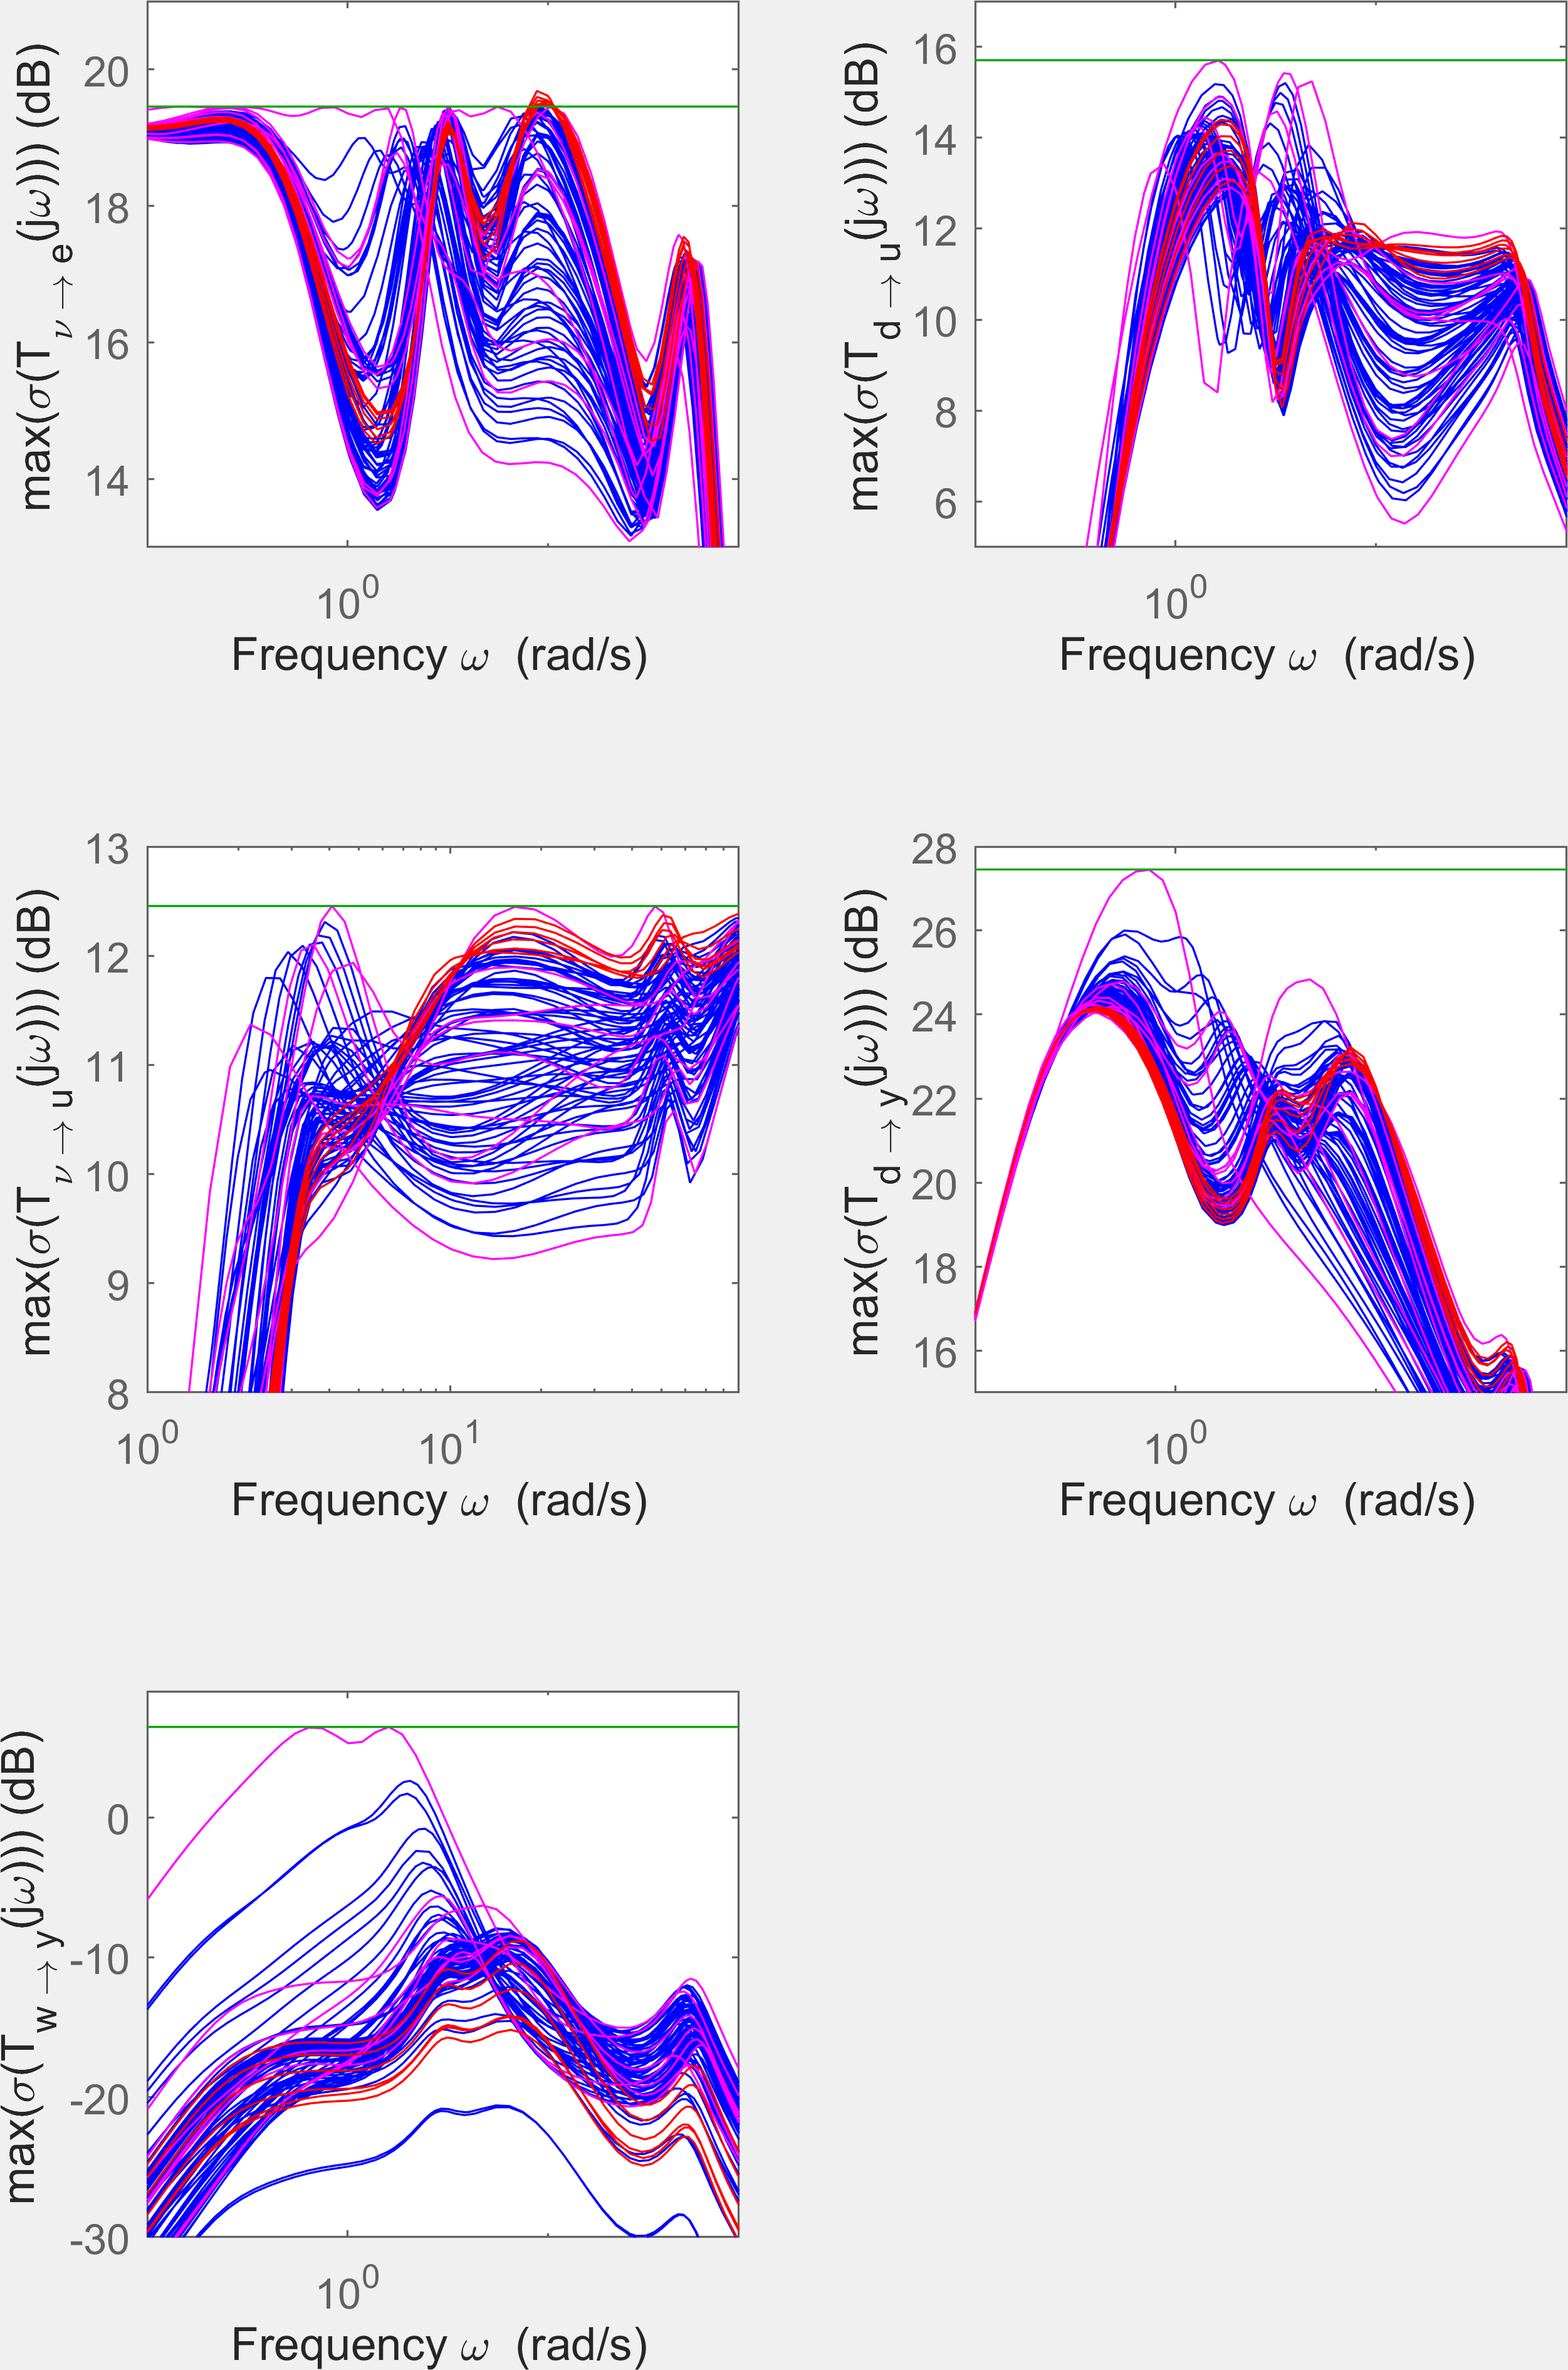
\includegraphics[trim=0cm 0cm 0cm 0cm,clip,width=0.9\columnwidth]{figures/transferts_tcst.png}
    \caption{Diagrams of the singular values of the transfer functions in \eqref{eq:validation_step} at the first iteration of Algorithm~\ref{alg:iterativeOptimisation}.}
    \label{fig:transferts_tcst}
\end{figure}


\begin{figure}[ht!]
    \centering
    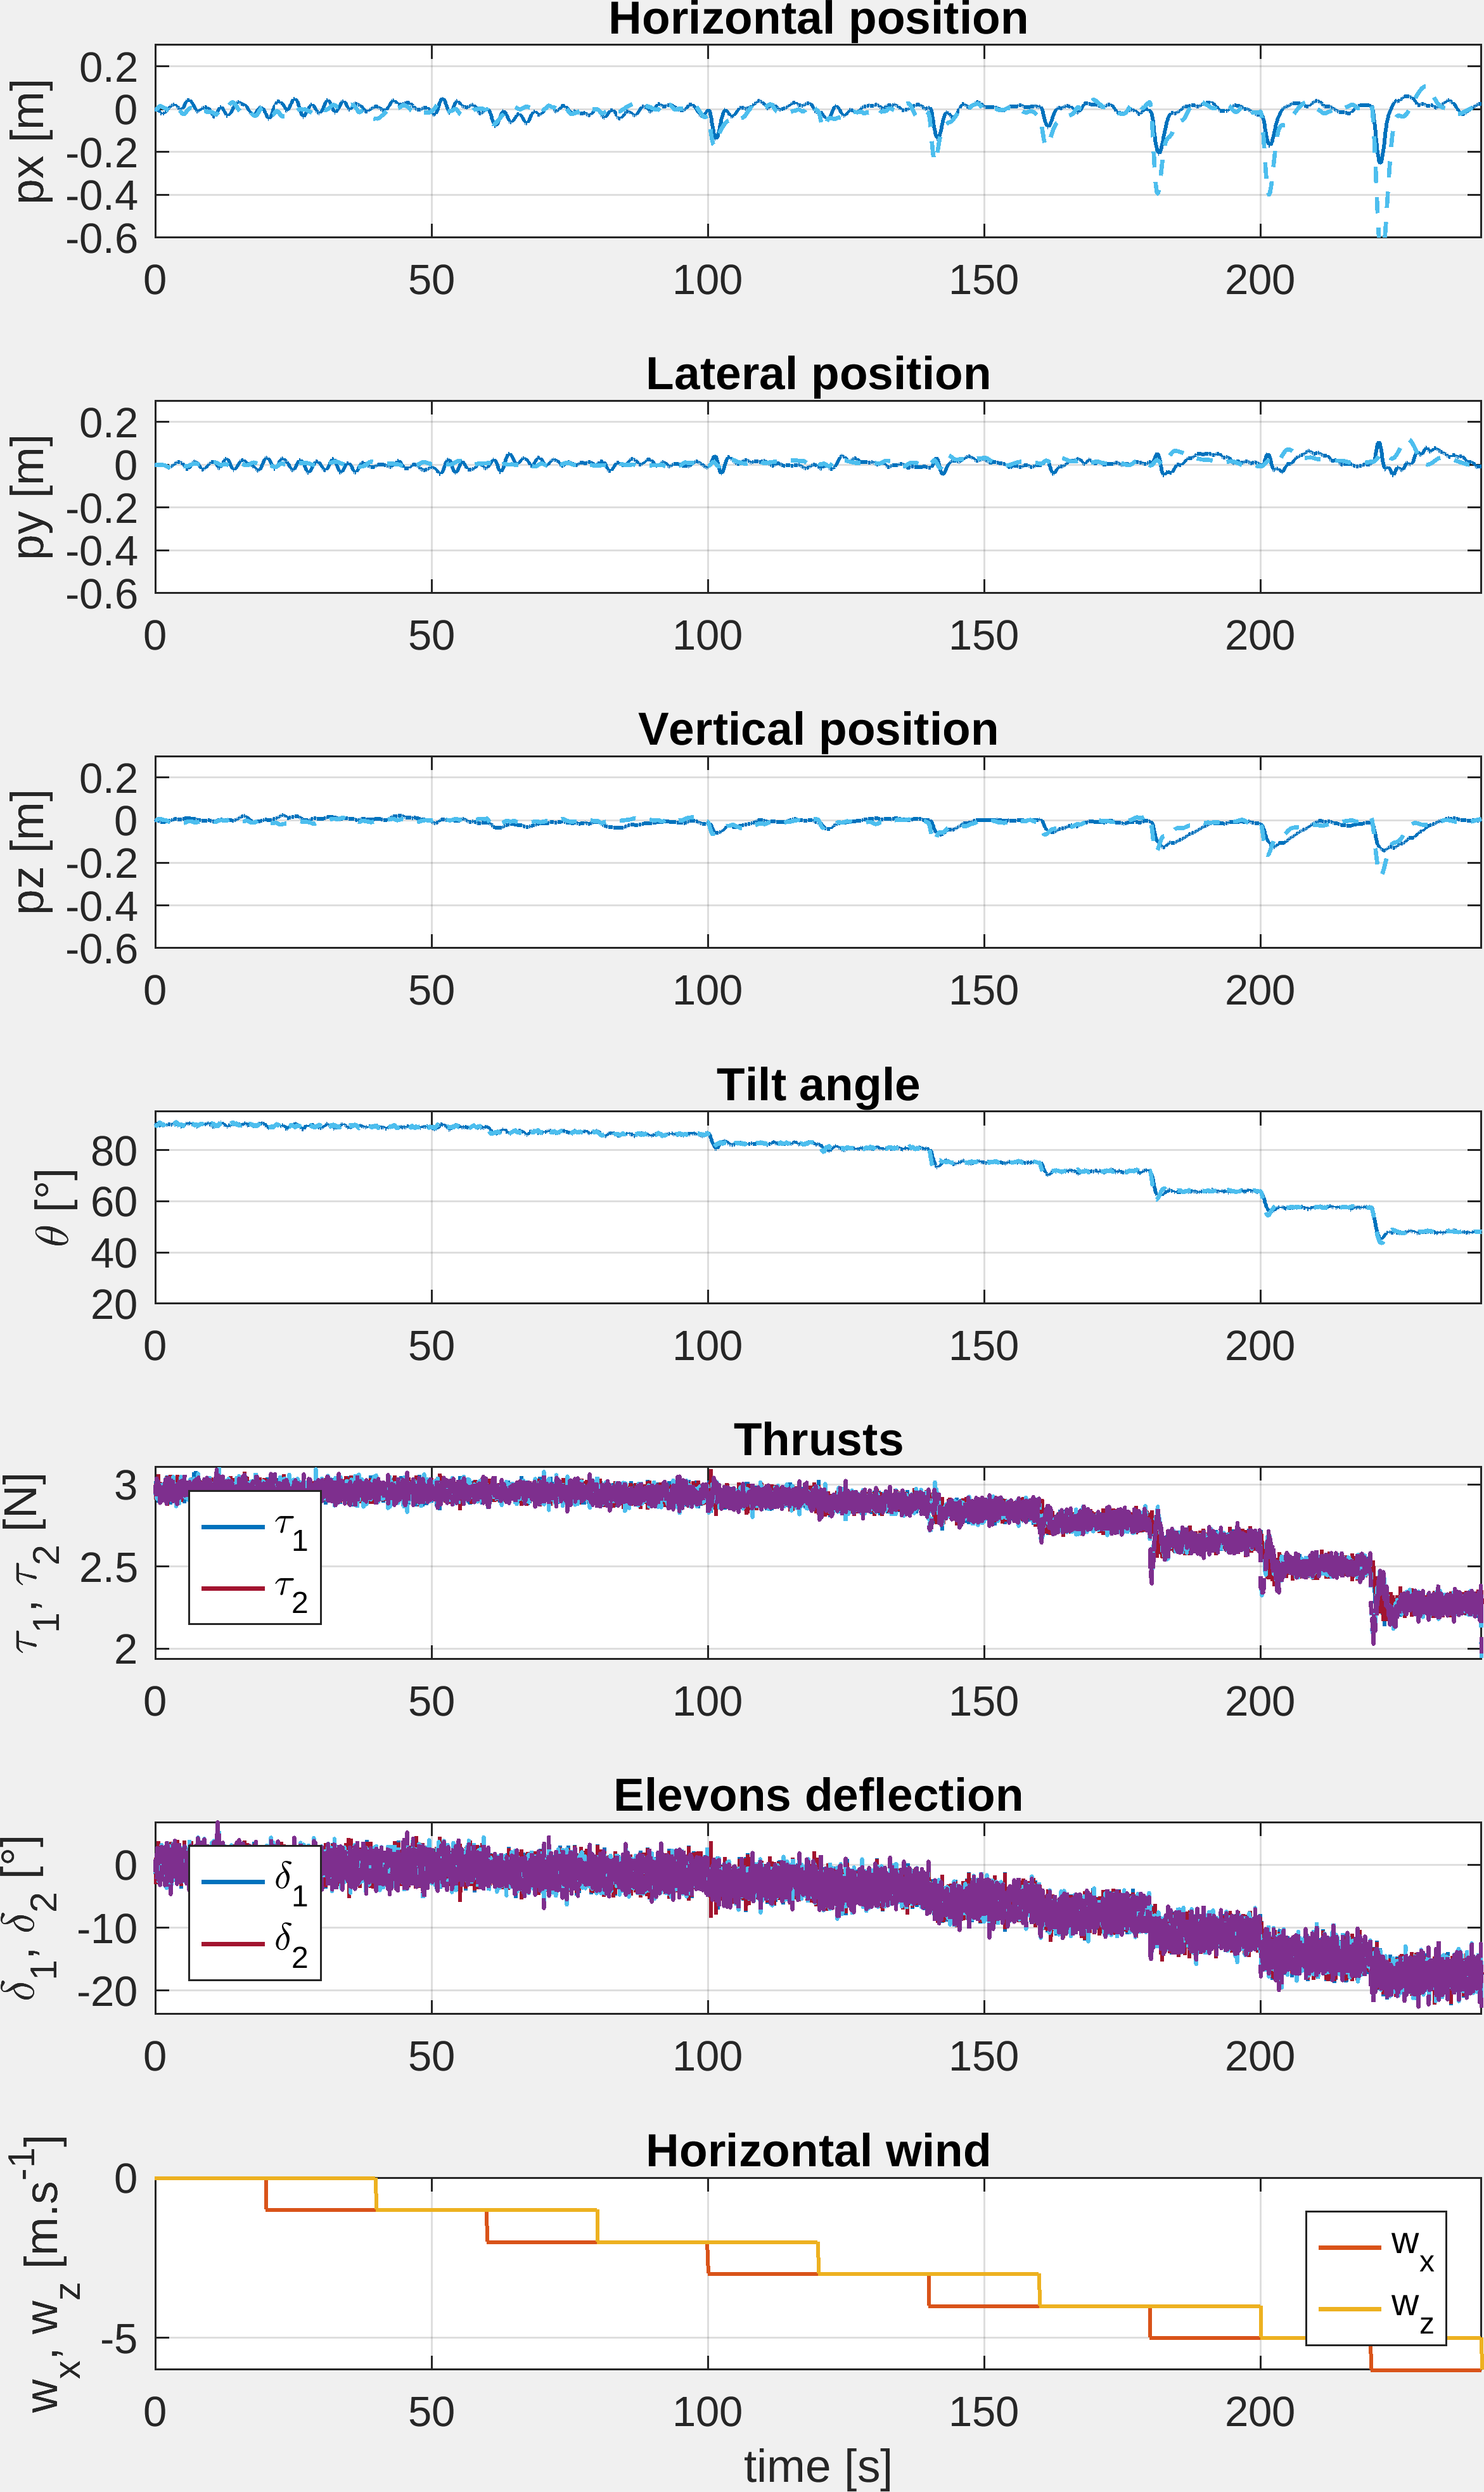
\includegraphics[trim=0cm 0cm 0cm 0cm,clip,width=0.9\columnwidth]{figures/sim_systune_lpv_noise.png}
    \caption{Simulation of the non-linear model \eqref{eq:dyna_orig} (solid line) and the linearized model  \eqref{eq:lpv_linearisation} (dashed line) with increasing constant wind steps with the controller tuned using the multimodel optimization of Algorithm~\ref{alg:iterativeOptimisation} in  Section~\ref{sec:h_inf_multi}.}
    \label{fig:SimSytuneStruct_lpv}
\end{figure}

With the tuning reported in \eqref{eq:gain_selection}, as obtained with Algorithm~\ref{alg:iterativeOptimisation}, we report in  Fig.~\ref{fig:SimSytuneStruct_lpv} parallel simulation results to those already shown in Fig.~\ref{fig:SimSytuneStruct_zero} for the zero-wind tuning method discussed in Section~\ref{sec:zerowind}. Once again we simulate both the nonlinear plant \eqref{eq:dyna_orig} (solid lines) and the linearized plant \eqref{eq:lpv_linearisation} (dashed line). 
As compared to Fig.~\ref{fig:SimSytuneStruct_zero}, the simulations of Fig.~\ref{fig:SimSytuneStruct_lpv} show that the controller tuning based on Theorems~\ref{thm:eqs} and~\ref{th:lin} 
solves the instability issues and manages to stabilize the hovering condition in all of the considered wind scenarios. We also note from 
Fig.~\ref{fig:SimSytuneStruct_lpv} shows a more aggressive action, indeed the control input $u$ (both thrust and deflections) is more affected by the measurement noise.
The effectiveness of the control scheme tuned on the basis of Algorithm~\ref{alg:iterativeOptimisation} is also confirmed by the experimental results reported in the next section.

% a larger stability range than in the case without wind (Fig.~\ref{fig:SimSytuneStruct_zero}), as we manage to stabilize the drone up to a vertical and horizontal speed of \SI{-6}{\meter\per\second}.


\section{Experimental flight with open wind tunnel} 
\label{sec:exp}
DarkO's experimental flight took place in a dedicated space (see Fig.~\ref{fig:flight_windshape}) with an Optitrack localization system based on a NED convention as per Figure~\ref{fig:darko2}. We used an open-vein wind generator to obtain wind steps that we measured with a hot-wire probe (the vertical bar in Fig.~\ref{fig:flight_windshape}). 
\begin{figure}[ht!]
    \centering
    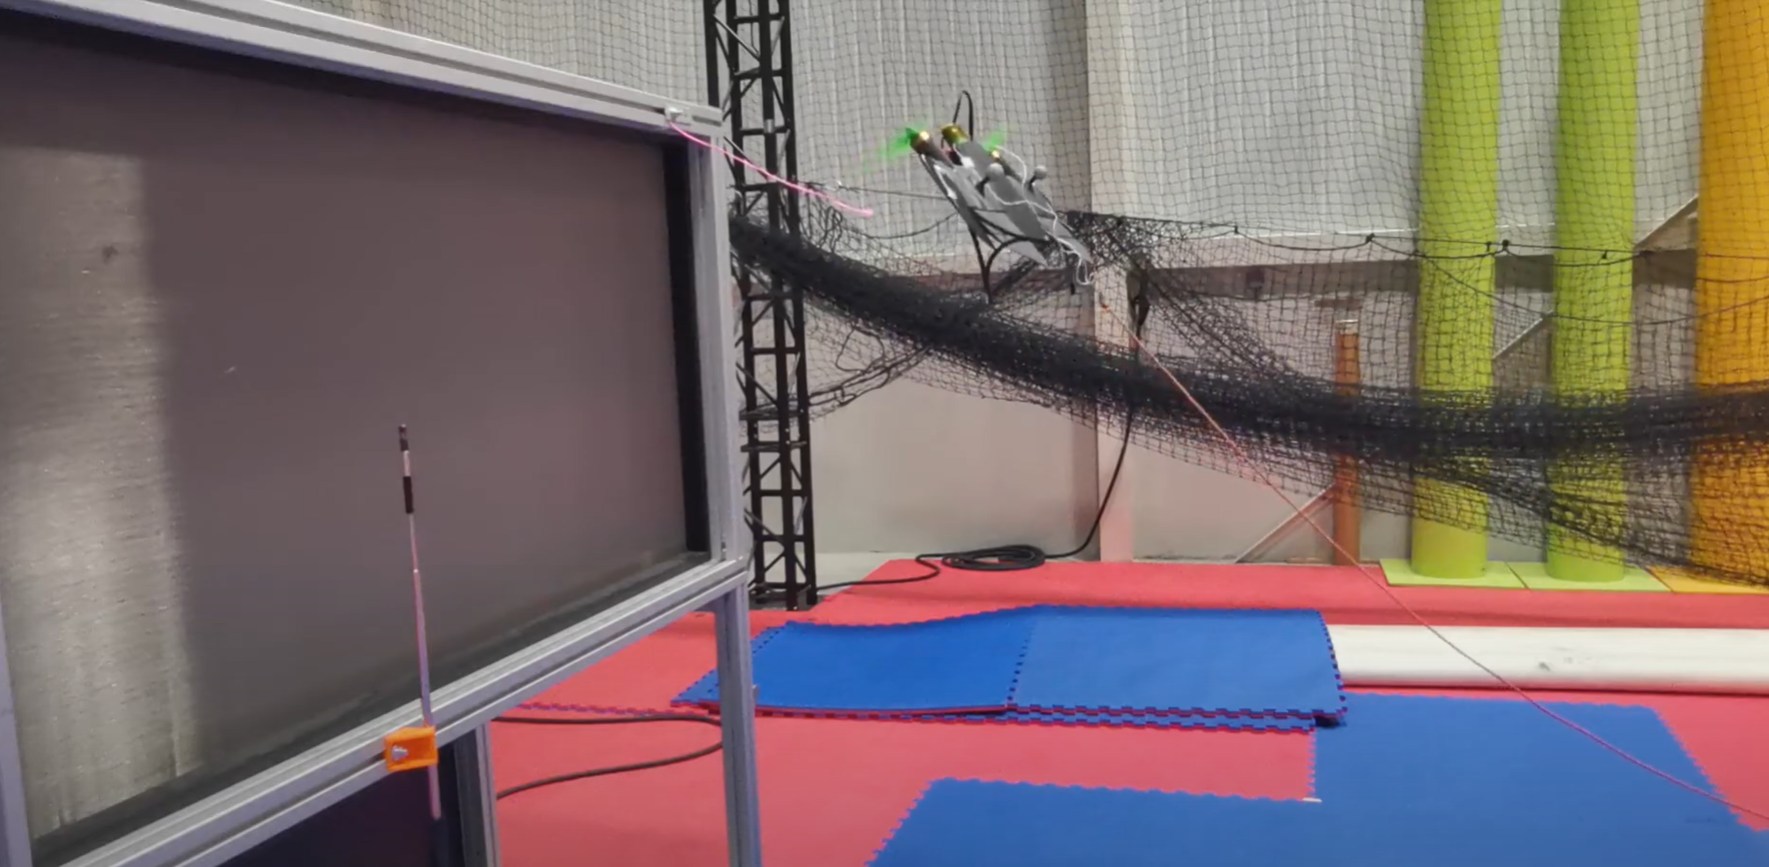
\includegraphics[trim=0cm 0cm 0cm 0cm,clip,width=1\columnwidth]{figures/img_flight_darko.png}
    \caption{DarkO's experimental flight in front of the open wind tunnel.}
    \label{fig:flight_windshape}
\end{figure}
Although this wind information is recorded on board the drone to synchronize the data, we do not use this measurement in the control law. The measurement frequency of this wind probe is only 0.5 Hz, so we only have one measurement every two seconds. 
The state estimation is carried out using an inertial navigation system to merge the Inertial Measurement Unit (IMU) + Optitrack sensor data in order to obtain an accurate estimation of the output $\boldsymbol{y}$ in Fig.~\ref{fig:commande_int}. However, the drone's angular velocity $\boldsymbol{\omega}_{\text{b}}$ is measured based on the IMU's gyrometer, which provides noisy measurements, therefore we added a second order Butterworth low-pass filter with cut-off frequency of 20 Hz to smoothen out the output $\boldsymbol{\omega}_{\text{b}}$. The Butterworth filter is considered in the linearized dynamics when optimizing the controller gains following Algorithm~\ref{alg:iterativeOptimisation}. 
\todo{comparaison lineaire}
\begin{figure}[ht!]
    \centering
    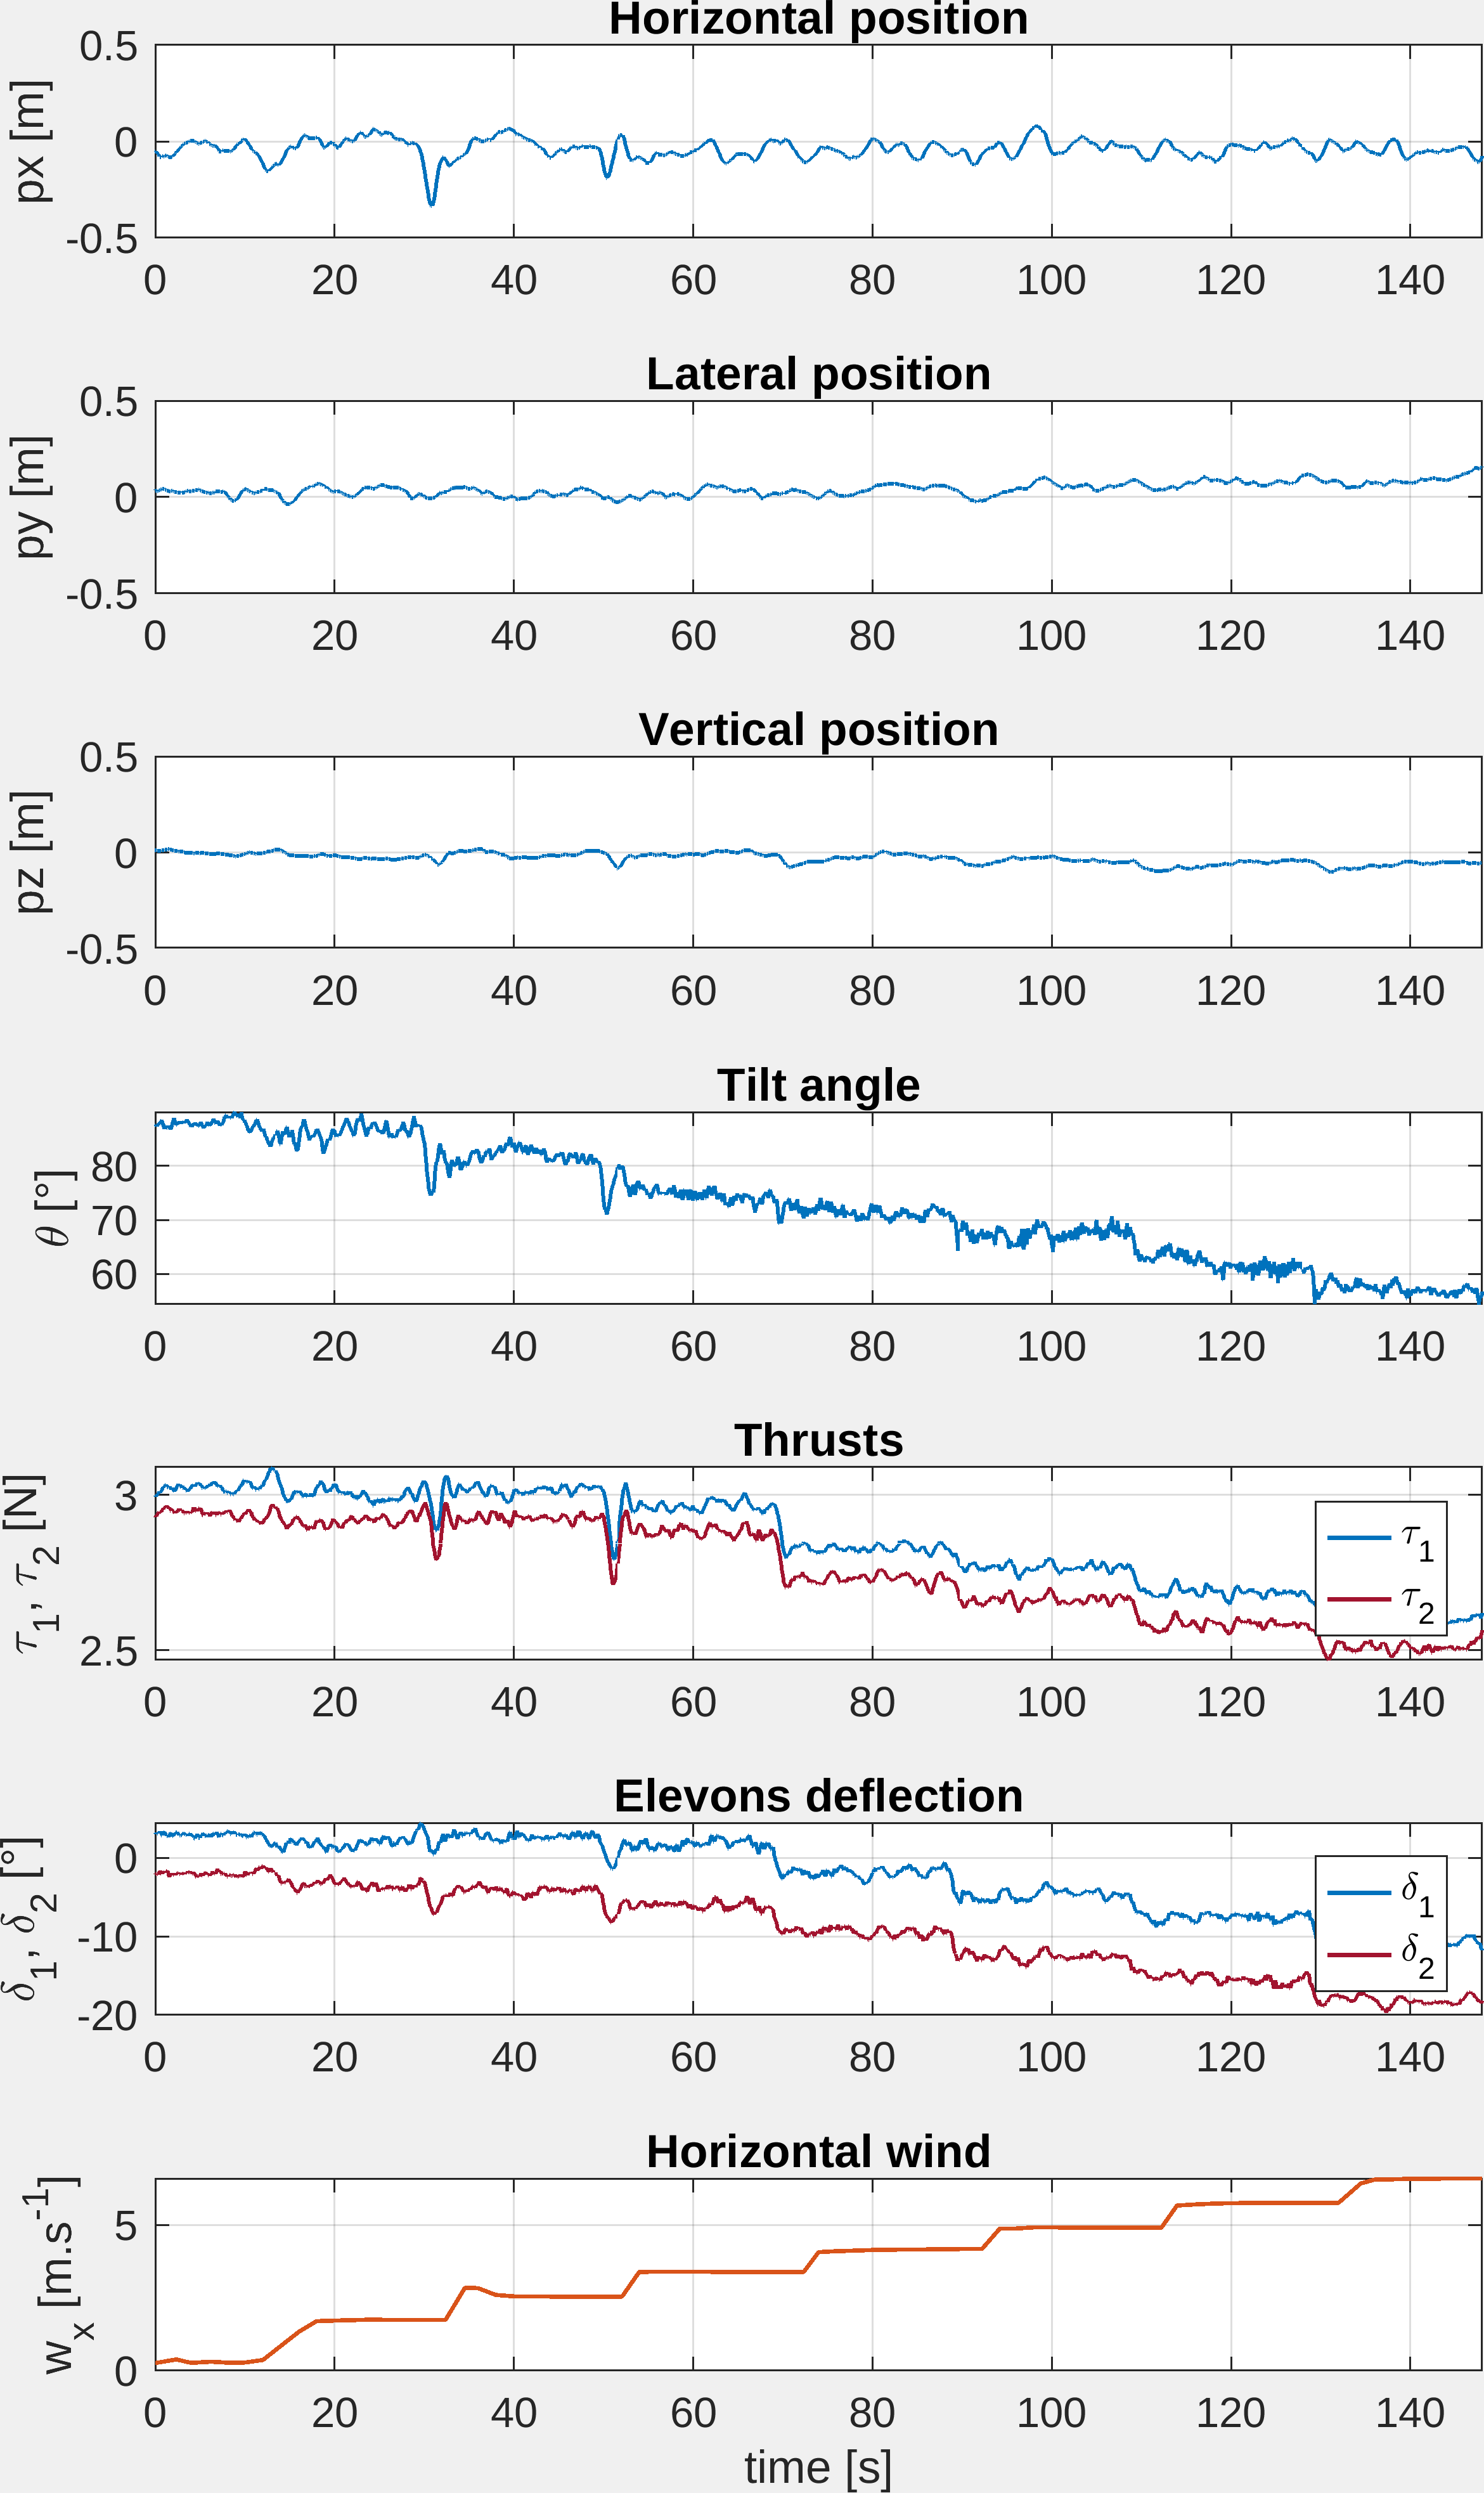
\includegraphics[trim=0cm 0cm 0cm 0cm,clip,width=0.9\columnwidth]{figures/exp_systune_struct.png}
    %'/home/florian/Log/DarkoLog/09_11_23/23_11_05__06_40_06_SD.data'
    \caption{Experiment of the DarkO UAV in front of the wind tunnel with increasing constant wind levels (lower plot).}
    \label{fig:ExpSytuneStruct}
\end{figure}

We also used the ESCs associated with the performance shown in Figure~\ref{fig:IOmot} for the propellers actuation. The two ESCs were flashed with the open-source code available in the GitHub repository AM32-MultiRotor-ESC-firmware\footnote{\url{https://github.com/FlorianSan/AM32-MultiRotor-ESC-firmware}}. The advantage of this firmware, as compared with the commercial code, is that it exploits a low-level PID feedback of the speed of rotation of the motor, which is calculated at the same speed as the motor phase commutation. We adapted the speed loop code in the firmware, following the approach of \cite{franchi2017}, featuring an adaptive bias and adaptive gain algorithm (ABAG). In this way, we compensate the battery discharge effects and obtain an accurate realization of the commanded speed. Before this modification, the integral action of the stabilizing feedback of Fig.~\ref{fig:commande_int} compensated for the motor speed loss caused by the battery voltage reduction during flight. This integral compensation was indirectly generated by the altitude loss of the UAV caused by the reduced traction. The advantages of the ABAG solution are high responsiveness and adaptability, as the propeller dimensions can be changed without needing to modify the actuation gains.

We carried out a flight experiment where DarkO was manually put into a stabilized hovering mode in front of the wind tunnel, then we switched on the control law of Algorithm~\ref{alg:iterativeOptimisation}. As the drone had to be stabilized at least \SI{30}{\centi\meter} away from the wind tunnel, a manual command was gradually applied to avoid overshooting, which could damage the wind tunnel. Once DarkO was close enough to the setpoint $\boldsymbol{r}_{p}$ of Fig.~\ref{fig:commande_int}, we switched on the proposed controller, obtaining the results in Fig.~\ref{fig:ExpSytuneStruct}. During the follow-up experimentation phase, as shown in the lower plot of Fig.~\ref{fig:ExpSytuneStruct}, we stepwise increased the wind speed, waiting 20 seconds between each  pair of consecutive steps, up to a final wind speed of \SI{7}{\meter\per\second}.

\begin{figure}[ht!]
    \centering
    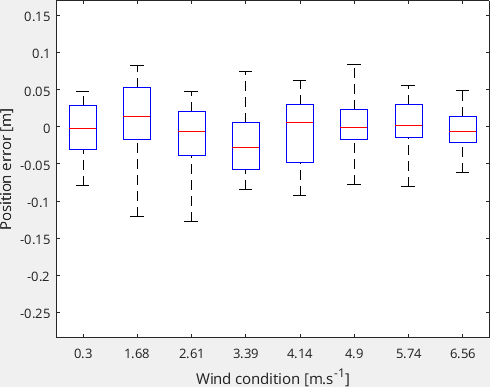
\includegraphics[trim=0cm 0cm 0cm 0cm,clip,width=0.9\columnwidth]{figures/boxplot.png}
    \caption{Statistical visualization of the hovering performance.}
    \label{fig:statpos}
\end{figure}
Figs~\ref{fig:ExpSytuneStruct} and~\ref{fig:statpos} show that the drone maintains its position despite the increasing wind speed. We can note a few important points, in agreement with the simulations: the motor traction decreases when increasing the wind speed. The control scheme takes advantage of the lift generated by the wind to support the drone, so that less energy is needed to stabilize the hovering position. The drone maintains its tilt angle at a value that is unknown a priori to the control law and naturally stems from the integral action that asymptotically attains the required value of the drone's pitch angle $\theta$. To stabilize the position, the UAV uses the elevons to cancel the pitch moment generated by the shape of the wing, subjected to a horizontal wind, without reaching the saturation limits.
We also notice a slight asymmetry of the effectiveness of the actuators, which is effectively compensated by the proportional action of the control scheme.
\section{Maquette expérimentale : 6 Dof}

\section{Résultats}






